\documentclass[a4paper]{scrartcl}
\usepackage{amsmath}
\usepackage{mathtools}
\usepackage{titlesec}
\usepackage[utf8]{inputenc}
\usepackage[polish]{babel}
\usepackage{textcomp}
\usepackage[T1]{fontenc}
\usepackage{amsthm}
\usepackage{amsfonts}

\title{Sieci komputerowe - warsztaty 7}
\author{Dawid Żywczak}
\date{10 czerwca 2020}

\begin{document}
\maketitle
\qquad Jako dowód wykonania zadania przesyłam zrzuty ekranu, tak jak ostatnio oraz postaram się odpowiedzieć na zadane pytania.\\
\section{Zadanie 1}
Pytania oraz odpowiedzi:\\
Na maszynie Virbian2 strumień danych występuje w postaci niezaszyfrowanej jako pakiety przesyłane z ::1:45032 do ::1:7777\\
Pomiędzy maszyną Virbian2 a maszyną Virbian1 strumień danych występuje w postaci zaszyfrowanej jako pakiety przesyłane z 192.168.1.2:42800 do 192.168.1.1:22.\\
Na maszynie Virbian1 strumień danych występuje w postaci niezaszyfrowanej jako pakiety przesyłane z 127.0.0.1:60180 do 127.0.0.1:7.
\begin{figure}
  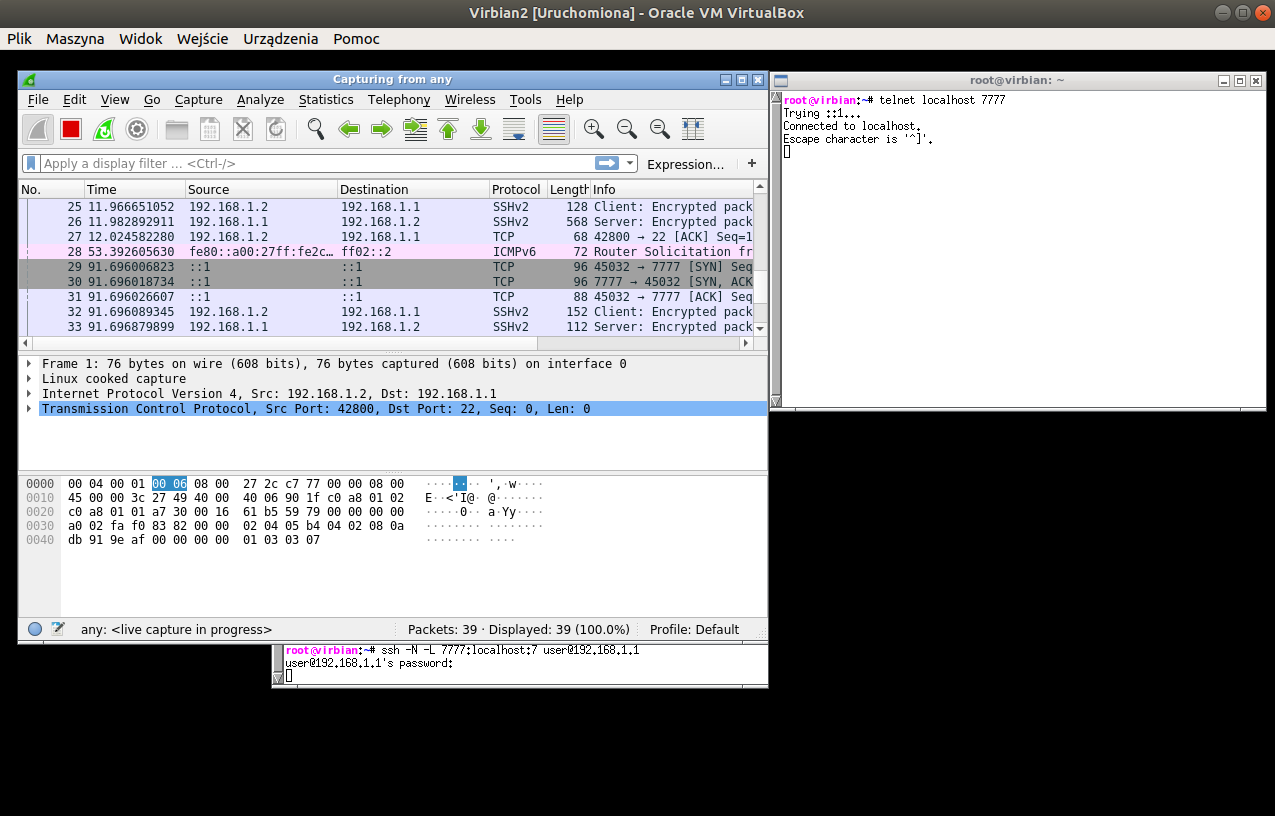
\includegraphics[width=\linewidth]{zad1.png}
  \caption{[Zadanie 1] Widok Wiresharka po wykonaniu polecenia w zadaniu na maszynie Virbian2}
\end{figure}
\begin{figure}
  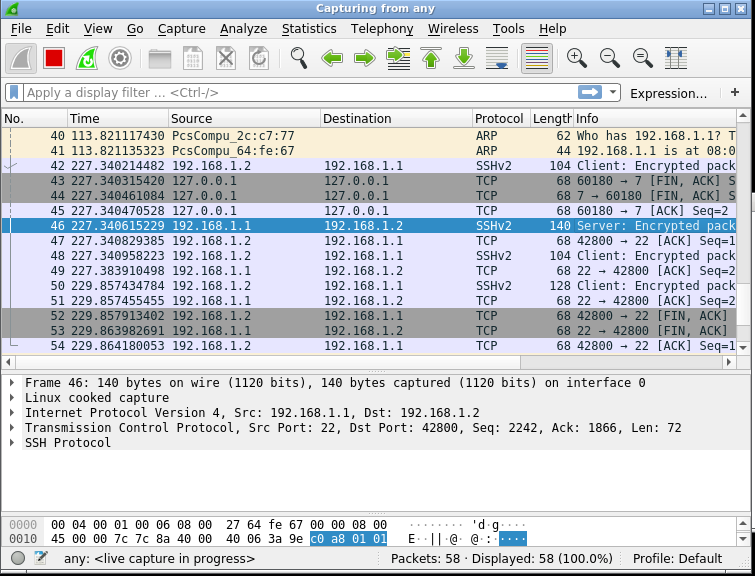
\includegraphics[width=\linewidth]{wireshark_v1.png}
  \caption{[Zadanie 1] Widok Wiresharka na maszynie Virbian1}
\end{figure}
\begin{figure}
  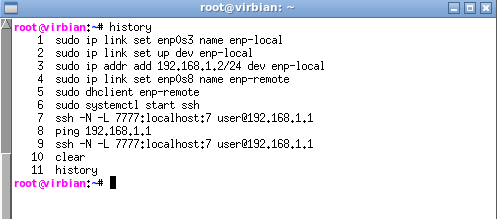
\includegraphics[width=\linewidth]{zad1_hist.png}
  \caption{[Zadanie 1] Historia terminala maszyny Virbian2 (maszyna Virbian1 została skonfigruowana zgodnie z zadaniem dopuszczającym do innych części)}
\end{figure}
\section{Zadanie 2}
Wykonanie zadania dokumentuję poprzez zrzuty ekranu terminali maszyn Virbian1 i Virbian2. Klucze podpisywane były zgodnie z tutorialem 2.
\begin{figure}
  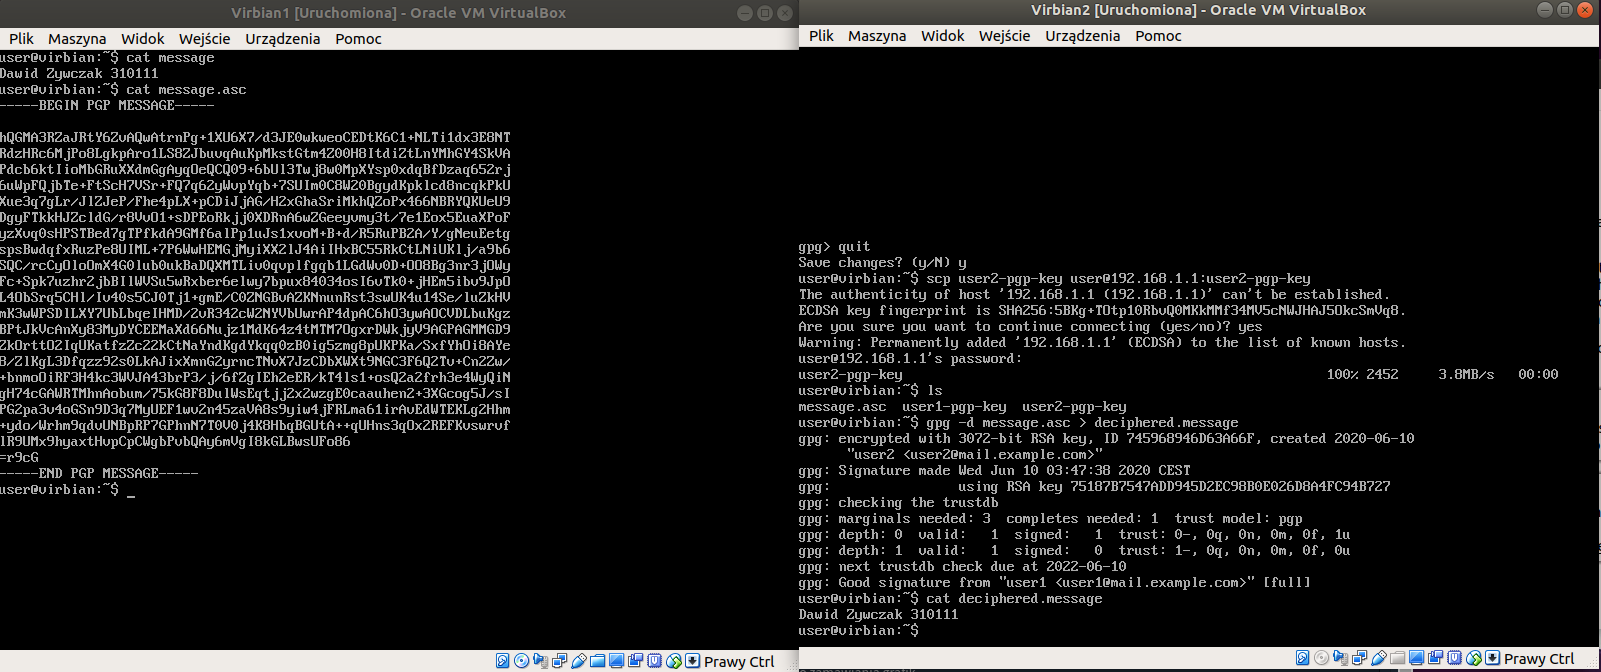
\includegraphics[width=\linewidth]{message.png}
  \caption{[Zadanie 2] Oryginalna oraz zaszyfrowana wiadomość na maszynie Virbian1 (po lewej stronie) oraz odszyfrowana wiadomość na maszynie Virbian2 (po prawej stronie)}
\end{figure}
\begin{figure}
  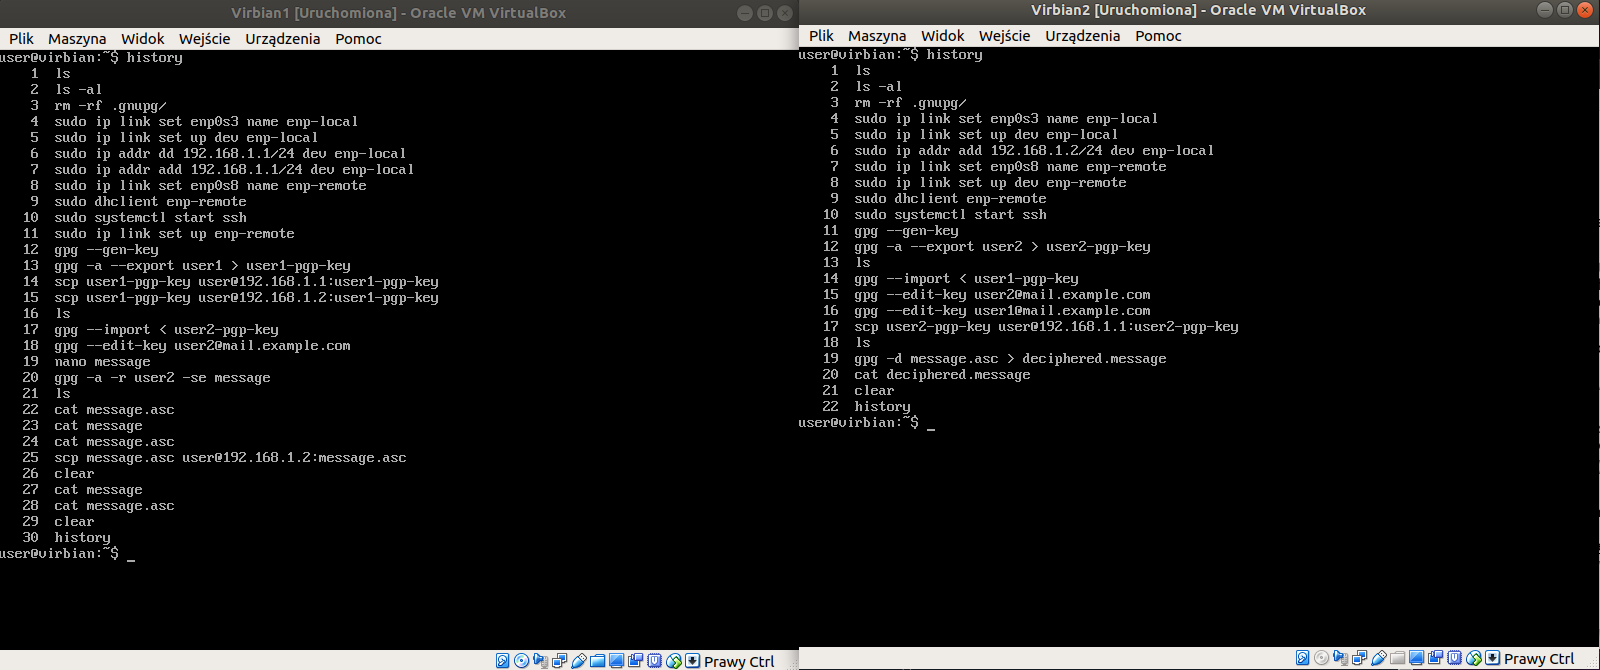
\includegraphics[width=\linewidth]{history.png}
  \caption{[Zadanie 2] Historia poleceń dla terminala w maszynie Virbian1 (lewa strona) i teminala w maszynie Virbian2 (prawa strona).}
\end{figure}
\end{document}